\section{姿勢制御系}

\subsection{制御方式}
OrigamiSat-1 搭載の 5.8GHz 通信用パッチアンテナは指向性を持つため,同アン
テナ取付面を地上に向ける姿勢制御が必要となる.本衛星では,永久磁石と地
磁気の干渉を利用した受動的姿勢制御を採用した.飛行と姿勢のイメージを図
\ref{image_attitude_ctrl}に示す.衛星内部に搭載された棒磁石により姿勢
は地磁場の磁力線に沿う様に回転する.この過程で,日本の緯度付近を通過す
る際,パッチアンテナの面が地上を向く.但し,軌道上では運動を減衰させる
要素が乏しく,実際には磁力線を中心に揺動運動することとなる.このため,
本衛星では,PCパーマロイ製のヒステリシスダンパを搭載している.本ダンパ
は,磁力線の相対運動に伴い電磁誘導を生じ,内部抵抗による電力消費によっ
て,運動を熱に変換する.本方式は,同じく5.8GHzパッチアンテナを搭載して
いた,FITSAT-1(にわか)に採用され,実績があることから採用した.

\begin{figure}[htbp]
	\centering
	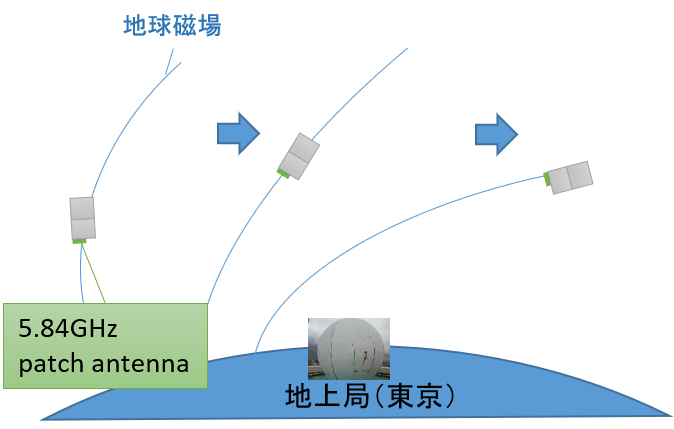
\includegraphics[width=10cm]{03/fig/image_attitude_ctrl.png}
	\caption{飛行と姿勢のイメージ}
	\label{image_attitude_ctrl}
\end{figure}

\subsection{主要諸元}
本衛星の姿勢制御用永久磁石およびヒステリシスダンパの搭載イメージを図
\ref{image_mag_HD}に示す.また,それぞれの諸元を表
\ref{spec_magnet}, 表\ref{spec_HD}に示す.

\begin{figure}[htbp]
	\centering
	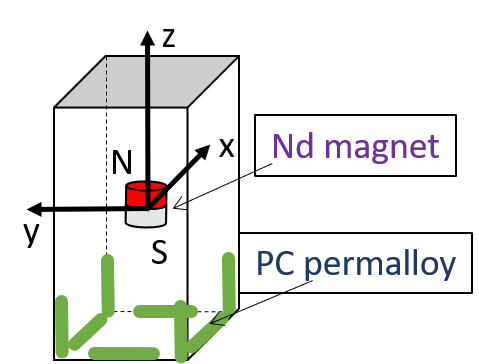
\includegraphics[width=5cm]{03/fig/image_mag_HD.png}
	\caption{永久磁石とヒステリシスダンパ搭載イメージ}
	\label{image_mag_HD}
\end{figure}

\begin{table}[htb]
    \centering
    \caption{OrigamiSat-1搭載磁石諸元}
    \begin{tabular}{cc} \hline
      項目 & 諸元 \\ \hline\hline
      材質 & Nd \\
        体積 & $2.73 \times 10^{-6} [\rm{m^3}]$\\ 
        磁束密度 & 0.468 [T] \\ 
        発生トルクオーダー & $10^{-5}$ [Nm] \\ \hline   
    \end{tabular}
    \label{requirment_op}
\end{table}

\begin{table}[htb]
    \centering
    \caption{OrigamiSat-1 搭載ヒステリシスダンパ諸元}
    \begin{tabular}{cc} \hline
      項目 & 諸元 \\ \hline\hline
        材質 & PC パーマロイ \\
        体積(X-axis) & 1.603 $\times 10^{-7} [\rm{m^3}]$ \\
        体積(Y-axis) & 1.320 $\times 10^{-7} [\rm{m^3}]$ \\
        体積(Z-axis) & 5.055 $\times 10^{-8} [\rm{m^3}]$ \\ 
        発生トルクオーダー & $10^{-6}$ [Nm] \\ \hline    
    \end{tabular}
    \label{requirment_op}
\end{table}



